%\newpage
% -----------------------------------------------------------------------
\chapter{Introduction and Overview}
%-----------------------------------------------------------------------
\section{Current Situation and Challenges}
\begin{itemize}
\item Software is ubiquitous.
\item Software is expensive. Cost for maintenance and support is much
higher compared to the development costs.
%\item Software ist teuer: Wartung und Unterhalt verursachen ein Mehrfaches der
%  Entwicklungkosten.
\item Building and maintaining software can be a risky business. Most
enterprises rely on software. Failure in development could therefore lead
to serious consequences. The top risks are
\begin{itemize}
\item Schedule (e.g. Time estimation)
\item Budget (e.g. Cost overrun)
\item Operational and Management (e.g. Resource planning)
\item Technical (e.g. Change of requirements)
\item External (e.g. Government rule change)
\end{itemize}

%\item Die Software-Entwicklung gehört zu den riskantesten
%  und anspruchsvollsten Vorhaben: häufige Termin- und
%  Kostenüberschreitungen, viele Projektscheiterungen, mangelhafte
%  Produkte, grosser
%  Verbesserungsbedarf \ldots

\item Rapid raising of software complexity. Today there are new technical
possibilities compared to what was possible a couple years age
(e.g. smart devices).

%\item Die Komplexität und der Funktionsumfang von Softwareprodukten nimmt
%  rasant zu. Heute sind Produkte erhältlich, die vor wenigen Jahren ausserhalb
%  des Machbaren lagen.
\end{itemize}
\subsection{Software Maintenance Cost}
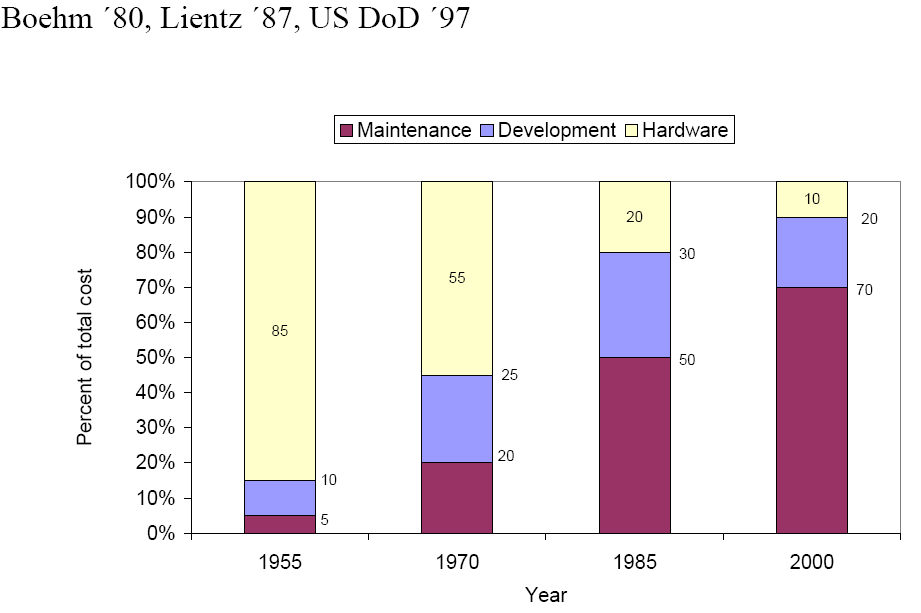
\includegraphics[width=\linewidth]{software-engineering/swMaintenanceCost}
%
\newpage
%\fi
\subsection{Standish Group Reports}
Based on more than 80000 software project there are the following comclusions:

%Anhand jährlicher Untersuchungen von mittlerweile über 80'000 kommerziellen
%Softwareprojekte werden die folgenden Schlussfolgerungen gezogen:

%(\href{http://www.standishgroup.com/sample_research/chaos_1994_1.php}
%  {www.standishgroup.com/sample\_research/chaos\_1994\_1.php}
%(\href{http://www.softwaremag.com/L.cfm?Doc=newsletter/2004-01-15/Standish}
%    {www.softwaremag.com/L.cfm?Doc=newsletter/2004-01-15/Standish})
\begin{center}
\begin{tabular}{lrr}
      & 1994 & 2004 \\
\hline
successful projects & 16 \% & 34 \%\\
 canceled software projects & 31 \% & 15 \% \\
cost of canceled software projects in Billion USD &  81  &  55\\
SW development cost in Billion USD &  250  &  255  \\
 average cost overrun & 180 \% & 43 \% \\
% Only 9\% of software projects for large companies were delivered
%  on time and within budget. For medium-sized and small companies, the
%  numbers improved to 16\% and 28\%, respectively.
\end{tabular}
\end{center}
\renewcommand{\arraystretch}{1.2}
\ifslides
{\footnotesize
\fi
\begin{tabular}[h]{lr|lr}
                  & \% OF &                        & \% OF \\
SUCCESSFUL PROJECTS & RESPONSES & CHALLENGED PROJECTS & RESPONSES \\
\hline
User involvement & 15.9 & Lack of user input & 12.8 \\
Executive mgmnt support & 13.9 & Incomplete requirements & 12.3 \\
Clear statement of requirements & 13.0 & Changing requirements & 11.8\\
Proper planning & 9.6 & Lack of executive support & 7.5 \\
Realistic expectations & 8.2 & Technology incompetence & 7.0 \\
Smaller project milestones & 7.7 & Lack of resources & 6.4 \\
Competent staff & 7.2 & Unrealistic expectations & 5.9 \\
Ownership & 5.3 & Unclear objectives & 5.3 \\
Clear vision and objectives & 2.9 & Unrealistic time frame & 4.3 \\
Hard-working, focused staff & 2.4 & New technology & 3.7 \\
Other & 13.9 & Other & 23.0 \\
\hline
\end{tabular}\\[2ex]
\ifslides
}
\fi
\begin{center}
\ifslides
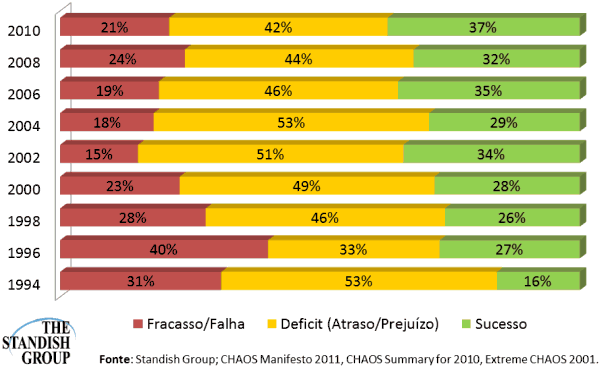
\includegraphics[width=0.9\linewidth]{software-engineering/standish_success_failure}
\else
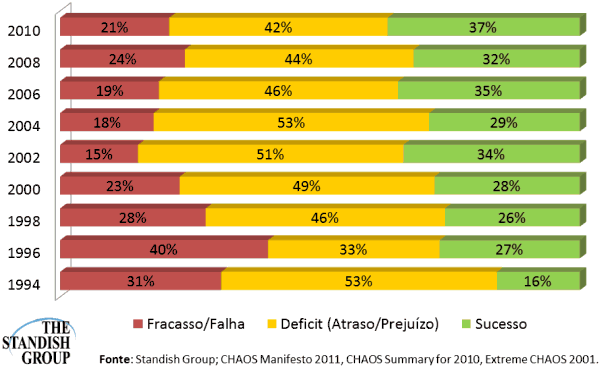
\includegraphics[width=0.6\linewidth]{software-engineering/standish_success_failure}
\fi
\end{center}
\ifslides
\newpage
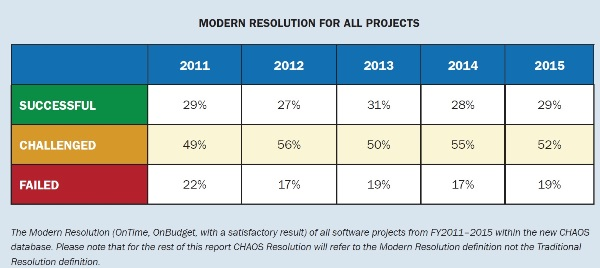
\includegraphics[width=\linewidth]{software-engineering/standish-1}
\newslide
\fi
  Research at the Standish Group also indicates that \hl{smaller time frames,
  with delivery of software components early and often, will increase the
  success rate}. Shorter time frames result in an iterative process
  of design, prototype, develop, test and deploy small elements. This
  process is known as growing software, as opposed to the old concept
  of developing software. Growing software engages the user earlier,
  each component has an owner or a small set of owners, and expectations
  are realistically set. In addition, each software component has a clear
  and precise statement and set of objectives. Software components
  and small projects tend to be less complex. Making the projects simpler
  as a worthwhile endeavor because complexity causes only confusion
  and increased cost.\\[2ex]
%-----------------------------------------------------------------------------
%\newpage
%\subsection{Definitionen}
%
\newpage
\section{Taking a Closer Look}
%\begin{description}
%\item[Systems-Engineering]
%Wegleitung, die auf bestimmten Denkmodellen und Grundprinzipien
%beruht, zur zweck\-m\"as\-si\-gen und zielgerichteten Gestaltung komplexer
%Systeme (W.F.Daenzer 1989).
%\item[Software] Die Programme, Verfahren, zugehörige Dokumentationen und
%  Daten, die mit dem Betrieb eines Computersystems zu tun haben (IEEE 610.12).
%\item[Software Engineering]
\structure{IEEE Standard Computer Dictionary} (Std 610):
\begin{quote}
(1) The application of a systematic, disciplined, quantifiable approach to the development,
   operation, and maintenance of software; that is, the application of engineering to software.

(2) The study of approaches as in (1)
\end{quote}
% Software Engineering Vocabulary:
%   https://pascal.computer.org/sev_display/index.action
%
% is the application of science and mathematics
%by which the capabilities of computer equipment
%are made useful to man via computer programs, procedures and associated
%documentation (B. Boehm 1981).
\newslide
\structure{Software Engineering Body of Knowledge} (SWEBOK V3):\\
%\href{https://www.computer.org/portal/web/swebok}{www.computer.org/portal/web/swebok}
\href{https://www.computer.org/education/bodies-of-knowledge/software-engineering}
  {www.computer.org/education/bodies-of-knowledge/software-engineering}
\ifslides

15 Knowledge Areas (KA) %Characterizing the Practice of Software Engineering:

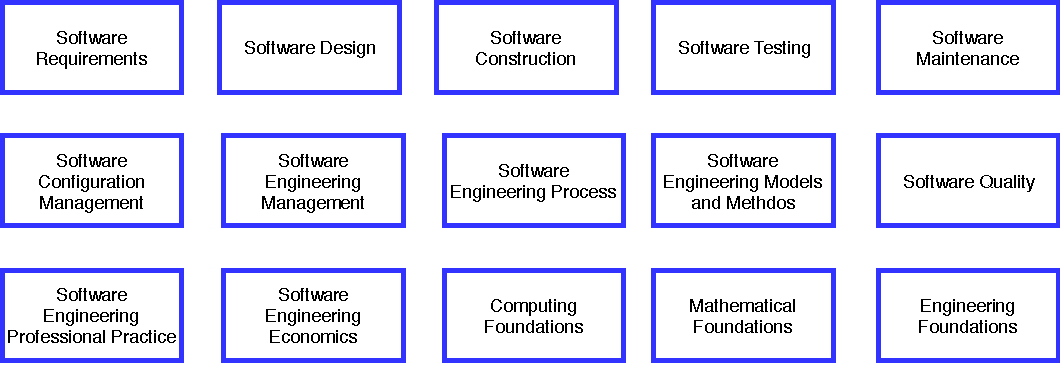
\includegraphics[width=\linewidth]{software-engineering/SWEBOK-KA}
\newslide
Covered in Modules Software Engineering% I / II:

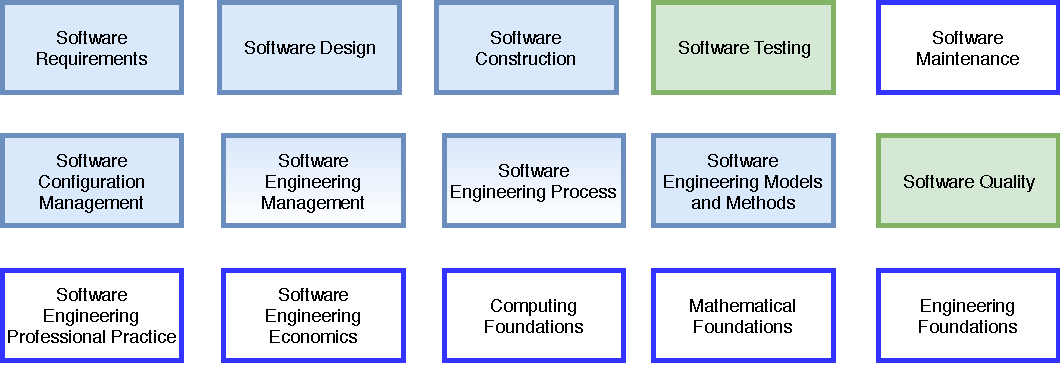
\includegraphics[width=\linewidth]{software-engineering/SWEBOK-KA2}
\newslide
\else
\begin{figure}[H]
  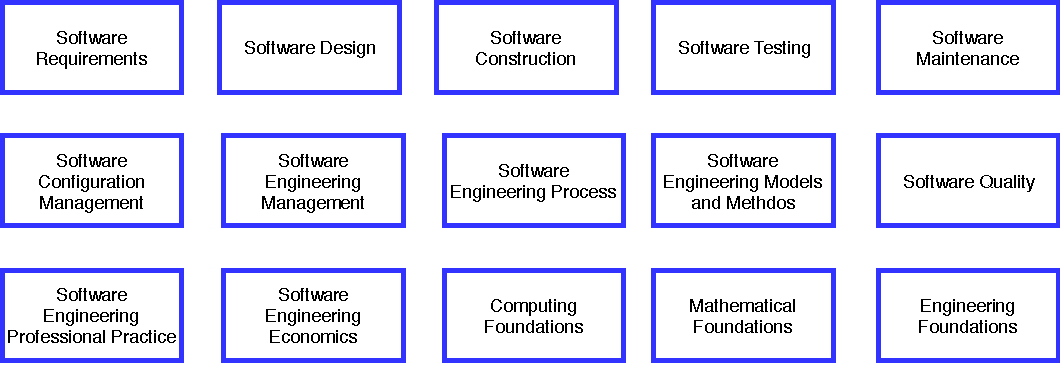
\includegraphics[width=\linewidth]{software-engineering/SWEBOK-KA}
  \caption{15 Knowledge Areas (KA)} %Characterizing the Practice of Software Engineering}
\end{figure}

\begin{minipage}{0.48\linewidth}
\fi
\begin{itemize}
\item \structure{Software Requirements}: elicitation, negotiation, analysis,
  specification, and validation,
  \item \structure{Software Design}: definition of the architecture, components, interfaces,
  \item \structure{Software construction}: detailed design, coding, unit testing,
    integration testing, debugging, verification and tools,
  \item \structure{Software Testing}: fundamentals of software testing; testing techniques;
    human-computer user interface testing and evaluation; test-related measures
  \item \structure{Software Maintenance}: program comprehension, re-engineering,
    reverse engineering, refactoring, software retirement; disaster recovery techniques, tools,
\newslide
\end{itemize}
\ifslides
\newslide
\else
\end{minipage}
\hfill
\begin{minipage}{0.48\linewidth}
\fi
\begin{itemize}
\item \structure{Software Configuration Management}: identification, control,
  status accounting, auditing; software release management and delivery, tools
\item \structure{Software Engineering Management}: process planning,
  estimation of effort, cost, and schedule, resource allocation, risk analysis,
  planning for quality;
  %software project enactment (measuring, reporting, and controlling; acquisition and supplier contract management);
  product acceptance; review and analysis of project performance; project closure; tools
\item \structure{Software Engineering Process}: software life cycle models,
  process assessment, tools
  \item \structure{Software Engineering Methods}: modeling, analysis %tools and methods
  \item \structure{Software quality}: verification, validation, reviews, audits, tools
\end{itemize}
\ifslides
\else
\end{minipage}
\hfill
\begin{minipage}[t]{0.48\linewidth}
\fi
\begin{itemize}
\item \structure{Software Engineering Professional Practice}:  standards,
  codes of ethics; group dynamics (working in teams, cognitive problem complexity,
  interacting with stakeholders, dealing with uncertainty and ambiguity,
  dealing with multicultural environments); communication skills
%\newslide
%\item Knowledge Areas Characterizing the Educational Requirements of Software Engineering
%  \begin{itemize}
\item \structure{Software Engineering Economics}: cost-benefit analysis,
  optimization, risk analysis, estimation, decision making
\end{itemize}
\ifslides
\else
\end{minipage}
\hfill
\begin{minipage}[t]{0.48\linewidth}
\fi
\begin{itemize}
\item \structure{Computing Foundations}: operation systems,
  networking, algorithms, parallel an distributed computing
\item \structure{Mathematical Foundations}: sets, relations, and
  functions; basic propositional and predicate logic;
  proof techniques; graphs and trees; discrete probability;
  grammars and finite state machines; and number theory.
\item \structure{Engineering Foundations}: statistical analysis;
  measurements and metrics; engineering design; simulation and modeling
\end{itemize}
\ifslides
\newslide
\else
\end{minipage}
\fi

\begin{minipage}{0.48\linewidth}
 7 Related Disciplines:
  \begin{itemize}
  \item Computer Engineering
  \item Computer Science
  \item General Management
  \item Mathematics
  \end{itemize}
\end{minipage}
\hfill
\begin{minipage}{0.48\linewidth}
  \begin{itemize}
  \item Project Management
  \item Quality Management
  \item Systems Engineering
  \end{itemize}
\end{minipage}
%\item[Projekt] ein zeitlich begrenztes, einmaliges Entwicklungsvorhaben zum
%L\"osen von Problemen innerhalb eines vorgegebenen Zielsystems. Es umfasst
%die Gesamtheit der f\"ur die Probleml\"osung notwendigen Entwicklungsarbeiten.
%\ifslides
%\newpage
%\fi
%\item[Projektmanagement] die Gesamtheit der organisatorischen und methodischen
%  Massnahmen zur ziel-, termin- und kostengerechten Abwicklung eines Projektes.
%
%  Dies umfasst (DIN 69 901):
%  \begin{itemize}
%    \item Führungsaufgaben: Zielsetzung,Zieleinhaltung, Entscheidung,
%    \item Führungsorganisation: Projektorganisation, Projektabwicklung,
%    \item Führungstechniken: Motivationstechnik, Besprechungstechnik,
%         Präsentationstechnik, Entscheidungsfindungstechnik
%    \item Führungsmitteln: Produkt- und Projektstrukturplanungssysteme,
%         Termin- / Kapazitäts-/ Kostenplanungs- und Steuerungssysteme
%       \end{itemize}
%
%
%\ifslides
%\newpage
%\fi
%   Die Ziele des Projektmanagements sind:
%\begin{itemize}
% \item Erstellen der erforderlichen Ergebnisse bzgl. Qualität und Funktion,
% \item     Reduzierung der Durchlaufzeit von Projekten,
%  \item     Reduzierung des Gesamtaufwands von Projekten,
%  \item     Erhöhung der Reaktionsfähigkeit der Projekte,
%  \item     Rechtzeitiges Erkennen und Vermindern von Risiken,
%  \item     Erhöhung der Transparenz über den Projektstand.
%  \end{itemize}
%\end{description}
\newpage
\subsection{Craft and Pragmatism}
Is software development more a \textcolor{blue}{\bfseries craft} than an \textcolor{OliveGreen}{\bfseries engineering} discipline?\\
(\href{http://www.developerdotstar.com/mag/articles/reeves_design.html}
{Jack W. Reeves, 1992})

Pragmatism considers words and thought as \hl{tools and instruments for prediction,
problem solving and action}, and rejects the idea that the function of thought is to
describe, represent, or mirror reality.

Pragmatists contend that most philosophical
topics—such as the nature of knowledge, language, concepts, meaning, belief, and
science—are all best viewed in terms of their \hl{practical uses and successes}.
%The philosophy of pragmatism ``emphasizes the practical application of ideas by acting on them to
%actually test them in human experiences''.
(\href{https://en.wikipedia.org/wiki/Pragmatism}{en.wikipedia.org/wiki/Pragmatism})

\newslide
{\bfseries Examples from The Pragmatic Programmer}\\
\href{https://blog.codinghorror.com/a-pragmatic-quick-reference}{blog.codinghorror.com/a-pragmatic-quick-reference}

%    Care About Your Craft
%    Why spend your life developing software unless you care about doing it well?
%
%    Think! About Your Work
%    Turn off the autopilot and take control. Constantly critique and appraise your work.
%
%    Provide Options, Don't Make Lame Excuses
%    Instead of excuses, provide options. Don't say it can't be done; explain what can be done.
\begin{itemize}
  \item \structure{Don't Gather Requirements – Dig for Them}
    Requirements rarely lie on the surface. They're buried deep beneath layers of assumptions, misconceptions, and politics.
  \item \structure{Work With a User to Think Like a User}
    It's the best way to gain insight into how the system will really be used.
  \item \structure{Program Close to the Problem Domain}
    Design and code in your user's language.
  \item \structure{Make Quality a Requirements Issue}
    Involve your users in determining the project's real quality requirements.
  \item \structure{There Are No Final Decisions}
    No decision is cast in stone. Instead, consider each as being written in the sand at the beach, and plan for change.
  \item \structure{Some Things Are Better Done than Described}
    Don't fall into the specification spiral – at some point you need to start coding.
  \item \structure{Don't Be a Slave to Formal Methods}
    Don't blindly adopt any technique without putting it into the context of your development practices and capabilities.
  \item \structure{Critically Analyze What You Read and Hear}
    Don't be swayed by vendors, media hype, or dogma. Analyze information in terms of you and your project.
%  \item
%    Costly Tools Don't Produce Better Designs\\
%    Beware of vendor hype, industry dogma, and the aura of the price tag. Judge tools on their merits.
  \item \structure{You Can't Write Perfect Software}
    Software can't be perfect. Protect your code and users from the inevitable errors.
\item \structure{Don't Live with Broken Windows}
    Fix bad designs, wrong decisions, and poor code when you see them.
%
%    Be a Catalyst for Change
%    You can't force change on people. Instead, show them how the future might be and help them participate in creating it.
%
%    Remember the Big Picture
%    Don't get so engrossed in the details that you forget to check what's happening around you.
%
%  \item
%    Invest Regularly in Your Knowledge Portfolio
%    Make learning a habit.
%  \item
%    It's Both What You Say and the Way You Say It
%    There's no point in having great ideas if you don't communicate them effectively.
  \item \structure{DRY – Don't Repeat Yourself}
    Every piece of knowledge must have a single, unambiguous, authoritative representation within a system.
%  \item
%    Make It Easy to Reuse
%    If it's easy to reuse, people will. Create an environment that supports reuse.
%
%    Eliminate Effects Between Unrelated Things
%    Design components that are self-contained. independent, and have a single, well-defined purpose.
%
%    Use Tracer Bullets to Find the Target
%    Tracer bullets let you home in on your target by trying things and seeing how close they land.
%
%  \item
%    Prototype to Learn
%    Prototyping is a learning experience. Its value lies not in the code you produce, but in the lessons you learn.
%  \item
%    Estimate to Avoid Surprises
%    Estimate before you start. You'll spot potential problems up front.
%  \item
%    Iterate the Schedule with the Code
%    Use experience you gain as you implement to refine the project time scales.
%
%    Keep Knowledge in Plain Text
%    Plain text won't become obsolete. It helps leverage your work and simplifies debugging and testing.
  \item \structure{Use the Power of Command Shells}
    Use the shell when graphical user interfaces don't cut it.
  \item \structure{Use a Single Editor Well}
    The editor should be an extension of your hand; make sure your editor is configurable, extensible, and programmable.
  \item \structure{Always Use Source Code Control}
    Source code control is a time machine for your work – you can go back.
%
%    Fix the Problem, Not the Blame
%    It doesn't really matter whether the bug is your fault or someone else's – it is still your problem, and it still needs to be fixed.
%
%    Don't Panic When Debugging
%    Take a deep breath and THINK! about what could be causing the bug.
%
%    "select" Isn't Broken.
%    It is rare to find a bug in the OS or the compiler, or even a third-party product or library. The bug is most likely in the application.
%
%    Don't Assume It – Prove It
%    Prove your assumptions in the actual environment – with real data and boundary conditions.
%
%    Learn a Text Manipulation Language.
%    You spend a large part of each day working with text. Why not have the computer do some of it for you?
%
%    Write Code That Writes Code
%    Code generators increase your productivity and help avoid duplication.
%
%    Design with Contracts
%    Use contracts to document and verify that code does no more and no less than it claims to do.

%    Crash Early
%    A dead program normally does a lot less damage than a crippled one.

%    Use Assertions to Prevent the Impossible
%    Assertions validate your assumptions. Use them to protect your code from an uncertain world.
%
%    Use Exceptions for Exceptional Problems
%    Exceptions can suffer from all the readability and maintainability problems of classic spaghetti code. Reserve exceptions for exceptional things.
%
%    Finish What You Start
%    Where possible, the routine or object that allocates a resource should be responsible for deallocating it.
  \item \structure{Minimize Coupling Between Modules}
    Avoid coupling by writing "shy" code and applying the Law of Demeter.
%
%    Configure, Don't Integrate
%    Implement technology choices for an application as configuration options, not through integration or engineering.
%
%    Put Abstractions in Code, Details in Metadata
%    Program for the general case, and put the specifics outside the compiled code base.
%
%    Analyze Workflow to Improve Concurrency
%    Exploit concurrency in your user's workflow.

%    Design Using Services
%    Design in terms of services – independent, concurrent objects behind well-defined, consistent interfaces.

%    Always Design for Concurrency
%    Allow for concurrency, and you'll design cleaner interfaces with fewer assumptions.
%  \item
%    Separate Views from Models\\
%    Gain flexibility at low cost by designing your application in terms of models and views.
%
%    Use Blackboards to Coordinate Workflow
%    Use blackboards to coordinate disparate facts and agents, while maintaining independence and isolation among participants.

%    Don't Program by Coincidence
%    Rely only on reliable things. Beware of accidental complexity, and don't confuse a happy coincidence with a purposeful plan.

%    Estimate the Order of Your Algorithms
%    Get a feel for how long things are likely to take before you write code.

%    Test Your Estimates
%    Mathematical analysis of algorithms doesn't tell you everything. Try timing your code in its target environment.
  \item \structure{Refactor Early, Refactor Often}
    Just as you might weed and rearrange a garden, rewrite, rework, and re-architect code when it needs it. Fix the root of the problem.
    \newslide
  \item \structure{Design to Test}
    Start thinking about testing before you write a line of code.
  \item \structure{Test Early. Test Often. Test Automatically}
    Tests that run with every build are much more effective than test plans that sit on a shelf.
%  \item
%    Test Your Software, or Your Users Will
%    Test ruthlessly. Don't make your users find bugs for you.
%
%    Don't Use Wizard Code You Don't Understand
%    Wizards can generate reams of code. Make sure you understand all of it before you incorporate it into your project.
%  \item
%    Abstractions Live Longer than Details\\
%    Invest in the abstraction, not the implementation. Abstractions can survive the barrage of changes from different implementations and new technologies.
%  \item
%    Use a Project Glossary
%    Create and maintain a single source of all the specific terms and vocabulary for a project.

%    Don't Think Outside the Box – Find the Box
%    When faced with an impossible problem, identify the real constraints. Ask yourself: "Does it have to be done this way? Does it have to be done at all?"

%    Start When You're Ready.
%    You've been building experience all your life. Don't ignore niggling doubts.
%  \item
%    Organize Teams Around Functionality
%    Don't separate designers from coders, testers from data modelers. Build teams the way you build code.
  \item \structure{Don't Use Manual Procedures}
    A shell script or batch file will execute the same instructions, in the same order, time after time.

%    Coding Ain't Done 'Til All the Tests Run
%    'Nuff said.

%    Use Saboteurs to Test Your Testing
%    Introduce bugs on purpose in a separate copy of the source to verify that testing will catch them.

%    Test State Coverage, Not Code Coverage
%    Identify and test significant program states. Just testing lines of code isn't enough.

%    Find Bugs Once
%    Once a human tester finds a bug, it should be the last time a human tester finds that bug. Automatic tests should check for it from then on.

%    English is Just a Programming Language
%    Write documents as you would write code: honor the DRY principle, use metadata, MVC, automatic generation, and so on.

%    Build Documentation In, Don't Bolt It On
%    Documentation created separately from code is less likely to be correct and up to date.

%    Gently Exceed Your Users' Expectations
%    Come to understand your users' expectations, then deliver just that little bit more.
  \item \structure{Sign Your Work}
    Craftsmen of an earlier age were proud to sign their work. You should be, too.
\end{itemize}
%
\subsection{A Simplified Model}
%\vfill
\begin{minipage}[t]{0.45\linewidth}
\textcolor{blue}{\large\bfseries Software Development}
\begin{description}
  \item[Requirements]: elicitation, negotiation, analysis, specification, and validation,
  \item[Design]: architecture, components, interfaces,
  \item[Construction]: coding, unit \& integration testing, documentation %integration testing, debugging,
\end{description}
\end{minipage}
\hfill
\begin{minipage}[t]{0.45\linewidth}
\textcolor{OliveGreen}{\large\bfseries Project Management:}
\begin{description}
\item[Configuration Management]: change control, release management
\item[Process Life Cycle]: planning, resource allocation, risk analysis
\item[Quality Management]: verification, validation, reviews
\end{description}
\end{minipage}

\section{Sample Software Projects}
\subsection{Ariane 5}
On June 4, 1996 an unmanned Ariane 5 rocket launched by the European Space
Agency exploded just forty seconds after its lift-off from Kourou, French
Guiana. The rocket was on its first voyage, after a decade of development
costing \verb|$|7 billion. The destroyed rocket and its cargo were valued at
\verb|$|500 million. A board of inquiry investigated the causes of the
explosion and in two weeks issued a report. It turned out that the cause
of the failure was a software error in the inertial reference system (IRS)
untested for use in a new launch environment.
Specifically a 64 bit floating point number relating to the horizontal
velocity of the rocket with respect to the platform was converted to a 16 bit
signed integer. The number was larger than 32767, the largest integer
storeable in a 16 bit signed integer, and thus the conversion failed.\\
(\href{http://www-users.math.umn.edu/~arnold/disasters/ariane.html}
{http://www-users.math.umn.edu/~arnold/disasters/ariane.html})

\section{Software Engineering in industrial automation management}
Software in the field of industrial automation include the
following:
\begin{itemize}
\item Condition monitoring for large machines
\item Measurement and control
\item Safety and security management
\end{itemize}

%TODO

\section{Software Engineering in health care and biomedicine}
Software in health care is incredibly diverse. There are
many different working environments:
\begin{itemize}
\item Creating and managing software systems that connect researchers with
clinical experiment data (e.g. clinical trial)
\item Developing mobile application to monitor and collect data of
patients (e.g. collecting data with a smart watch).
\item Providing health care providers with data records about a
patient (e.g. doctor appointment).
\item Implement software systems which allows the handling of big data sets (
e.g. creating new software to predict skin cancer based on historical data).
\item Implement software systems for embedded devices (
e.g. software for a ventilator)
).
\item Implement software systems to support any health care environment (
e.g. electronic lab journal).
\item ... and many more
\end{itemize}

There are several aspects which must be considered:

\begin{itemize}
\item Data Security: handling of patient data
\item Reliability: devices are responsible for the health of patients
(e.g. a ventilator)
\item Traceability: Each change in a system must be documented
(e.g. which input data and source code was used to create the output data)
\end{itemize}

\section{Exercises}
\begin{enumerate}
\item What are the basic tasks that all software engineering projects must handle?
\item List five tasks that might be part of software deployment and explain why.
\item Collect several reasons why software engineering projects could fail.
\end{enumerate}

%
